\subsubsection{Freedom Board}
Das Freedomboard wurde im C Kurs getestet auf seine Grundfunktionen.
Insbesondere die Kommunikation über UART wurde ausgiebig verwendet
\cite{ninuxC}. Ein Beispiel hierfüg ist die Ansteuerung einer RGB LED
per UART wie im folgenden Programmabschnitt dargestellt.

\lstinputlisting[firstline=82, lastline=102, title=
	Main-Routine einer einfachen Kommandoverarbeitung]{coding/main.c}

In einem weiteren Versuch ist mit dem CodeWarrior ein I$^2$C Schnittstelle
initialisiert und mit einem LogicAnalyzer geprüft worden. Dieser Versuch ist
in Zusammenarbeit mit dem Elektrotechniker des Teams 31 durchgeführt worden.
Hierbei ist das Freedomboard als Master und ein Mototrenteiber-PCB von
Adafruit als Slave einesetzt worden. Das Ergebnis einer Kommunikation ist
in der Abbildung \ref{fig:frdm-i2c} dargestellt.

\begin{figure}[h!]
	\centering
	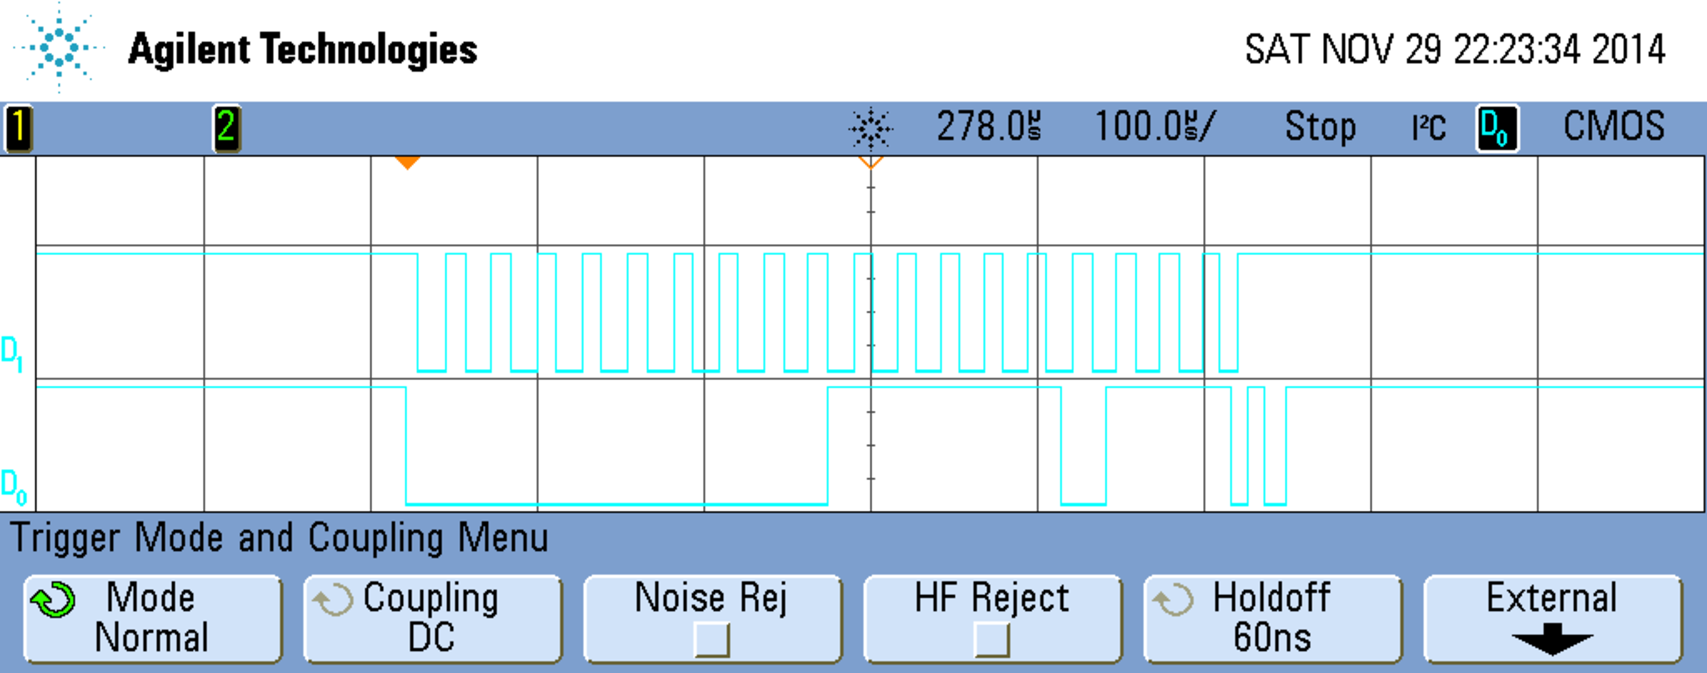
\includegraphics[width=0.75\textwidth]{../../fig/frdm-i2c_crop.pdf}
	\caption{I$^2$C Kommunikation (D$_1$: SCL, D$_2$: SDL)}
	\label{fig:frdm-i2c}
\end{figure}
